\documentclass[hidelinks,12pt]{article}
\usepackage{graphicx}
\usepackage{hyperref}
\usepackage{xcolor}


\title{Quantum Machine Learning}
\author{Hamza, Ali; Hoda, Bilal}
\date{\today}

\begin{document}

\maketitle

\begin{center}
    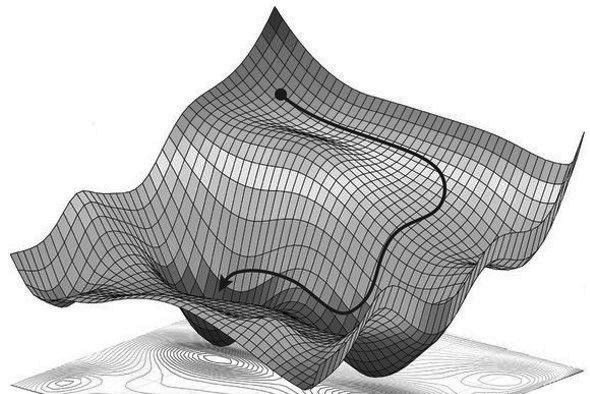
\includegraphics[scale = 0.7]{images/title2.jpg}
\end{center}
\newpage

\tableofcontents
\newpage

\section{Abstract}
\newpage
\section{Introduction}
\subsection{What is Machine Learning?}

	\hspace{0.5cm}The data that we observe can be generally explained by an underlying process.
	However, we might not know the details of this process underlying the generation of data. For instance, consumer behavior, we know is not completely random. People do not go to supermarkets and buy things at random. Do they buy then buy ice cream in summer or hot beverages in winters. There are certain patterns in the data.[1]
	\paragraph{}
	It is possible, that we may not be able to identify the process completely, but a good and useful approximation can be constructed. That approximation may not things completely, but may be able to account for some part of the data. We acknowledge that even though identifying the complete process may not be possible, certain regularities or patterns can still be detected. This is where machine learning comes in. These regularities or patterns may help us understand the process, or we can use those patterns to make predictions, by working with the assumption that at least the near future, will not be very different from what has been observed in the past when the sample data was collected.[1]
	\paragraph{}
	\textit{Machine Learning (ML)} is the field of study that involves techniques that give the ability to machines to learn from past experience. Typical tasks in Machine Learning may include predicting some unobserved characteristic (regression) or the class (classification) of an object based on some observations in the supervised learning, or the ability to find some structure hidden within data (density estimation or clustering) in unsupervised learning. Generally in Machine Learning, a machine is trained using a learning algorithm that takes as input a training data-set. In the context of classical computing this training data-set is implicitly assumed to be classical, meaning that it contains “classical” observations about “classical” objects.[2]
	\paragraph{}
	Based on learning methods, Machine Learning is generally divided into three categories. The first category is \textit{Supervised learning}. Supervised learning problems are those in which the training data comprises examples of the input vectors along with their corresponding target vectors.The digit recognition example, in which the aim is to assign each input vector to one of a finite number of discrete categories, is called a classification problem. If the output that we are trying to obtain consists of one or more continuous variables, then the task is called regression. Prediction of the yield in a chemical manufacturing process in which the input features consist of the concentrations of reactants, the temperature, and the pressure is an example of regression.[1]
	\paragraph{}
	In \textit{Unsupervised learning} problems the training data consists of a set of input vectors x without any corresponding target values. The goal may be to discover groups of similar examples within the data, where it is called clustering, or to determine the distribution of data within the input space, known as density estimation, or to project the data from a high-dimensional space down to two or three dimensions for the purpose of visualization.[1]
	\paragraph{}
	Finally, \textit{Reinforcement learning} is concerned with the problem of finding suitable actions to take in a given situation in order to maximize a reward. In reinforcement learning the algorithm is not given examples of optimal outputs, in contrast to supervised learning, but must instead discover them by a process of trial and error. There is a sequence of states and actions in which the learning algorithm is interacting with its environment. In many cases, the current action not only affects the immediate reward but also has an impact on the reward at all subsequent time steps. For instance, by using appropriate reinforcement learning techniques a neural network can learn to play the game of backgammon to a high standard. Here the network must learn to take a board position as input, along with the result of a dice throw, and produce a strong move as the output. This is done by having the network play against a copy of itself for a large number of games.[1]

\subsection{What is Quantum Machine Learning?}

\newpage
\section{Classical Machine Learning Algorithms}
\subsection{Gradient Descent}

	Machine Learning often relies on optimization to obtain results that are to make use of complex classification problems, such as curve fitting, pattern recognition, etc. These are built upon a cost/loss function that makes use of the present data. The purpose of a cost function is to optimize the present function so that it presents us with the most accurate classification of the data. \texit{Gradient Descent}.
	\paragraph{}
	Gradient Descent uses approximation and calculus to find the global extremes of a function, $f(x)$, where $x$ is an N-Dimensional vector. The purpose of using gradient descent instead of differentiation is simple. Not all curves are well defined functions and thus through a simple recursive algorithm, finding the extreme values of the curve become relatively easy. 
	\paragraph{}
	Let us begin by making use of analogy. Suppose you're at the top of the mountain and want to get to the bottom in the least amount of steps. Since you're in a 3D space, you can only move in the x, y or some combination of the two vectors. Through, Gradient Descent you can find the best step which has the highest rate of decrease in altitude. This process is then repeated until the decrease caused by the steepest step is approaches a very small value $\approx 0$ [12]
	\paragraph{}
	[12] The mathematical definition of this algorithm is as follows:  
	$$f(x_i, y_i) = f(x_{i-1}, y_{i-1} - \alpha\nabla f(x_{i-1}, y_{i-1})$$


\subsection{Support Vector Machines}
	The support vector machines algorithm (SVM) is a supervised machine learning algorithm used for linear discrimination problems. Our goal is to find an optimal hyperplane which maximizes the margin such that it discriminates between classes of feature vectors and is used as a decision boundary for future data classification. The SVM is formulated as maximizing
	the distance between the hyperplane and closest data points called support vectors. The objective function could be convex or non-convex depending on the kernel used in SVM algorithm.[3]

	\begin{center}
	    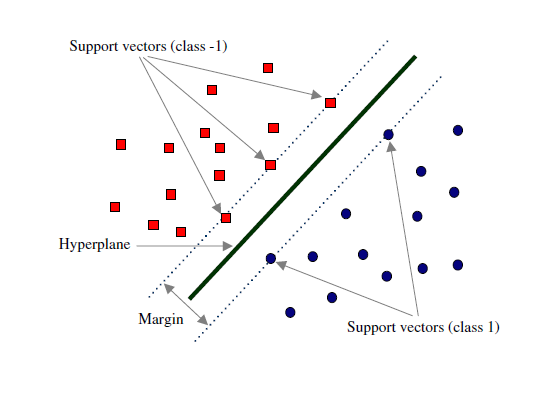
\includegraphics[scale = 0.7]{images/hyperplane.png}
	    Figure: Hyperplane [4]
	\end{center}

	We have l training examples where each example x are of D dimension and each have labels of either y=+1 or y= -1 class, and our examples are linearly separable. Then, our training data is of the form,
	\begin{center}
	    $\{x_i,y_i\}$ where i = 1 ... L, $y_i \in \{-1,1\}$, x $\in$ $R^D$ 
	\end{center}

	If the number of input features is 2, then the hyperplane is just a line. If the number of input features is 3, then the hyperplane becomes a two-dimensional plane. It becomes difficult to visualize when the number of features exceeds 3.
	Support vectors are data points that are closer to the hyperplane and influence the position and orientation of the hyperplane. Using these support vectors, we maximize the margin of the classifier. Deleting the support vectors will change the position of the hyperplane.[5]
	\\

	We define a linear discriminate function as;
	\begin{center}
	y = f(x) = w. x + b     
	\end{center}
	where w is the p-dimensional weight vector which is perpendicular to the hyperplane and b is a scalar which is the bias term.  Adding the offset parameter b allows us to increase the margin. If b is absent, then
	the hyperplane is forced to pass through the origin, restricting the solution. 
	The hyperplanes in the image can be described by equation: 
	\begin{center}
	    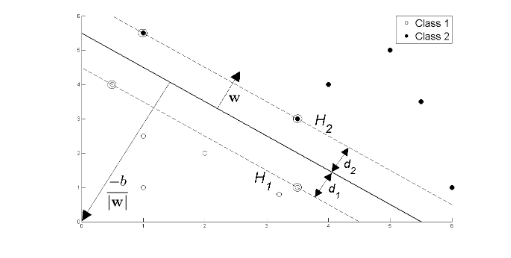
\includegraphics[scale = 0.7]{images/svm.png}
	    Figure: Hyperplane [4]
	\end{center}
	\begin{center}
	$w.x_i + b \geq +1$  for $y_i$=+1\\
	$w.x_i + b \leq -1 $ for $y_i$=-1    
	\end{center}
	We combine above two equations and we get;
	\begin{center}
	$y_i(w.x_i + b)-1 \geq 0$  for $y_i$=+1,-1\\
	\end{center}

	The two hyperplane H1 and H2 passing through the support vectors of +1 and -1 class respectively, so:
	\begin{center}
	w.x+b=-1 :H1\\
	w.x+b=1 :H2    
	\end{center}
	The distance between H1 hyperplane and origin is $\frac{(-1-b)}{|w|}$ and distance between H2 hyperplane and origin is $\frac{(1-b)}{|w|}$. So, margin can be given as
	\begin{center}
	M=$\frac{(1-b)}{|w|}$ - $\frac{(-1-b)}{|w|}$\\
	M=$\frac{2}{|w|}$
	\end{center}
	Where M is nothing but twice of the margin. So margin can be written as $\frac{1}{|w|}$. As, optimal hyperplane maximize the margin, then the SVM objective is boiled down to fact of maximizing the term $\frac{1}{|w|}$,
	Maximizing this term is equivalent to saying we are minimizing $|w|$ i.e. ( min($|w|$))
	or we can say min($\frac{||w||^2}{2}$) such that $y_i(w.x_i + b)-1 \geq 0$ for i =1...l

	SVM optimization problem is a case of constrained optimization problem, and it is always preferred to use dual optimization algorithm to solve such constrained optimization problem. That’s why we don’t use gradient descent.

	Lagrange method is required to convert constrained optimization problem into an unconstrained optimization problem. The goal of the above equation is to get the optimal value for w and b. So using Lagrange multipliers we can write the above expression as;
	\begin{center}
	    L = $\frac{||w||^2}{2} - \sum_{i=1}^{l} \lambda_i(y_i(w\cdot x_i+b)-1)$\\
	\end{center}
	\begin{equation}
	            L = \frac{||w||^2}{2} - \sum_{i=1}^{l} \lambda_i(y_i(w\cdot x_i+b))-\sum_{i=1}^{l}\lambda_i
	\end{equation}
	Now, we take the partial derivative of it with respect to w, b and $\lambda$.
	\begin{center}
	        $\frac{\partial l}{\partial w}$ = $w - \sum_{i=1}^{l} \lambda_i y_i x_i=0$\\
	        $\frac{\partial l}{\partial \lambda}$ = $ \sum_{i=1}^{l} y_i (w \cdot x_i+b)-1=0$\\
	        $\frac{\partial l}{\partial b}$ = $ \sum_{i=1}^{l} \lambda_i \cdot y_i=0$
	\end{center}
	From above we get:
	\begin{center}
	        w = $\sum_{i=1}^{l} \lambda_i y_i x_i$\\
	        $ \sum_{i=1}^{l} \lambda_i \cdot y_i=0$
	\end{center}

	From the above formulation we are able to find the optimal values of w only and it is dependent on $\lambda$, so we need to  also find the optimal value of $\lambda$. Finding the optimal value of b needs both w and $\lambda$. Hence, finding the value of $\lambda$ is important for us. Therefore, we do some algebraic manipulation:
	\\

	We substitute the value of w into equation 1. 

	\begin{center}
	$L_d = \frac{ (\sum_{i=1}^l\lambda_i \cdot y_i \cdot x_i)(\sum_{j=1}^l\lambda_j \cdot y_j \cdot x_j)}{2}-\sum_{j=1}^l\sum_{i=1}^l\lambda_j y_j(||\lambda_i \cdot y_i \cdot x_i||.x_j+b)+\sum_{i=1}^l \lambda_i$
	\end{center}
	\begin{center}
	    $L_d$ =$ \frac{(\sum_{i=1}^l\lambda_i \cdot y_i \cdot x_i)(\sum_{j=1}^l\lambda_j \cdot y_j \cdot x_j)}{2}-\sum_{j=1}^l\sum_{i=1}^l\lambda_j\lambda_i y_j y_i x_j x_i+\sum_{j=1}^l\sum_{i=1}^l\lambda_j y_j b+\sum_{i=1}^l \lambda_i$
	\end{center}
	Since our constraint was $\lambda_j \geq 0$ and $\sum_{j=1}^l\sum_{i=1}^l\lambda_j y_j$=0 so that term becomes zero. The first two terms get subtracted and after simplifying we have:
	\begin{center}
	    $L_d$ =$ \sum_{i=1}^l \lambda_i-\frac{1}{2}\sum_{j=1}^l\sum_{i=1}^l\lambda_j\lambda_i y_j y_i x_j x_i$
	\end{center}
	The optimization depends on the dot product of pairs of samples i.e. $x_i \cdot x_j$

	Now if the samples of our classes are not linearly separable then we transform our vectors to some other space and maximize the dot product of the transformation $\phi(x_j)\cdot\phi(x_i)$. Alternatively we use a function $K(x_i,x_j)=\phi(x_i)\cdot\phi(x_j)$ such that we don't need to know the transformation and this function gives us the dot product of the transformations in some space. This function in the context of SVMs is called a Kernel Function.
	\begin{center}
	    $L_d$ =$ \sum_{i=1}^l \lambda_i-\frac{1}{2}\sum_{j=1}^l\sum_{i=1}^l\lambda_j\lambda_i y_j y_i K(x_i, x_j)$
	\end{center}
	There are many kernel functions in SVM, so how to select a good kernel function is also a research issue. However, for general purposes, there are some popular kernel functions:
	\\

	1. Linear kernel: $K (x_i , x_j) = x_i^T\cdot x_j$ 

	2. Polynomial kernel: $K (x_i , x_j) = (\gamma x_i^T x_j + r)^d , \gamma > 0$ 

	3. RBF Kernel: $ K (x_i , x_j) = exp(-\gamma ||x_i - x_j||^2) , \gamma > 0$

	4.Sigmoid kernel:$ K (x_i , x_j) = tanh(\gamma x_i^T x_j + r)$  

	Here, $\gamma$, r and d are kernel parameters.[6]

\newpage
\section{Quantum Machine Learning Algorithms}
\subsection{Quantum Gradient Descent}
\subsection{Support Vector Machines via Grover's Algorithm}
We discussed above, An SVM is a supervised learning model that classifies data into one of the two given categories. In particular, an SVM provides a decision boundary with margin to each category of data as large as possible. In particular, an SVM provides a decision boundary with margin to each
category of data as large as possible. Implementing SVMs using quantum algorithms can result in significant speedup over the classical implementations, potentially bringing the originally polynomial complexity down
to logarithmic scale.
\newpage
\section{Quantum Neural Networks}
\newpage
\section{Reflection}
\subsection{Advantages of Quantum Machine Learning}
\subsection{Current Limitations}
\subsection{Future Prospects}
\newpage
\section{Bibliography}
\begin{enumerate}
    \item \url{https://kkpatel7.files.wordpress.com/2015/04/alppaydin_machinelearning_2010.pdf}
    \item \url{https://www.researchgate.net/publication/225151243_Machine_Learning_in_a_Quantum_World}
    \item \url{https://arxiv.org/pdf/1804.10068.pdf}
    \item \url{https://medium.com/@ankitnitjsr13/math-behind-support-vector-machine-svm-5e7376d0ee4d}
    \item \url{https://towardsdatascience.com/support-vector-machine-introduction-to-machine-learning-algorithms-934a444fca47}
    \item \url{http://www.jatit.org/volumes/research-papers/Vol12No1/1Vol12No1.pdf?fbclid=IwAR0xhouaOTffxsjwMCONzZeOubmQWl3PfZH94AUXMCNbfpBWKQaDbSBefNI}
    \item \url{https://arxiv.org/pdf/1909.05074.pdf}
    \item \url{https://arxiv.org/pdf/1909.02108.pdf}
    \item \url{https://arxiv.org/pdf/0905.2794.pdf}
    \item \url{https://iopscience.iop.org/article/10.1088/1367-2630/ab2a9e/pdf}
    \item Peter Wittek - Quantum Machine Learning - What Quantum Computing Means to Data Mining-Elsevier AP, Academic Press (2014)
    \item Understanding Machine Learning From Theory to Algorithms by Shalev-Shwartz S., Ben-David S.
    \
\end{enumerate}



\end{document}